\textbf{Aufgabe 1:}\newline
$\begin{array}{lrcl}
	I&(x+1)(x-1)&\leq&0\\
	II&\sqrt{x}&\geq&1
\end{array}$\newline
\newline
Ungleichung 1 wird nach dem Umstellen zu :

\begin{center}
	$x^2\leq 1$
\end{center}

\noindent Woraus sich die L�sungsmenge $L_1=\lbrace x\in \R\mid -1\leq x\leq 1\rbrace$ ergibt.\newline
Aus Ungleichung II ergibt sich nur die L�sung 

\begin{center}
	$x\geq 1$
\end{center}

\noindent ergibt. Somit ist $L_2=\lbrace x\in R\mid x\geq 1$.\newline
Als Gesamtl�sung ergibt sich $L=L_1\cap L_2=\lbrace x\in\R\mid x=1\rbrace$.\newline
\newline
\textbf{Aufgabe 2:}\newline
$\sqrt{\frac{1}{2}x^3+2x^2+\frac{21}{8}x+\frac{9}{8}}<\sqrt{\frac{1}{2}x^2+\frac{3}{2}x+\frac{9}{8}}$\newline
Ich nehme an, dass hier gewollt ist, dass man beide Seiten quadriert, was analytisch dann mit einer Vierfachunterscheidung gehen w�rde, die Ersties laut den vorherigen Seiten aber nicht tun d�rfen. Da ich aber auch keine andere L�sung sehe, tu ich das hier einfach mal:

$\begin{array}{crcl}
	&\frac{1}{2}x^3+2x^2+\frac{21}{8}x+\frac{9}{8}&<&\frac{1}{2}x^2+\frac{3}{2}x+\frac{9}{8}\\
	\Rightarrow&\frac{1}{2}x^3+\frac{3}{2}x^2-\frac{3}{8}x&<&0\\
	\Rightarrow&\frac{1}{2}x(x^2+3x-\frac{3}{4})&<&0
\end{array}$\newline
\newline
Mit Hife der Berechnung der Nullstellen, kann man die Intervalle angeben, in denen die Ungleichung gilt. Die Nullstelle $x_1=0$ ist offensichtlich. Nun noch die anderen beiden:\newline
\newline
$\begin{array}{crcl}
	&x_{2,3}=-\frac{3}{2}\pm\sqrt{\frac{9}{4}+\frac{3}{4}}\\
	\Rightarrow&x_{2,3}=-\frac{3}{2}\pm\sqrt{3}
\end{array}$\newline
\newline
Mit den Nullstellen gibt es f�r den Graphen 2 Alternativen, wie er aussehen kann:

\includegraphics[scale=1]{img/ungleichungen_aufg2.jpg}

Mit der Berechnung von f(-1) bekommt man dann auch raus, welcher der beiden Graphen auf unsere Ungleichung zutrifft:

\begin{center}
	$f(-1)=\frac{11}{8}$
\end{center}

\noindent Somit ist die L�sungsmenge $L=\lbrace x\in\R\mid x<-\frac{3}{2}-\sqrt{3}\vee 0<x<-\frac{3}{2}+\sqrt{3}\rbrace$.\newline
\newline
\textbf{Aufgabe 3:}
\begin{center}
	$x^2>2$
\end{center}

\noindent Es ergibt sich direkt die L�sungsmenge $L=\lbrace x\in \R\mid x<-\sqrt{2}\vee x>\sqrt{2}\rbrace$\newline
\newline
\textbf{Aufgabe 4:}
\begin{center}
	$x^3+3x^2-4>0$
\end{center}

\noindent Man berechne wieder die Nullstellen: $x_1=1;x_{2,3}=-2$. Wieder ergeben sich 2 m�gliche Graphen:
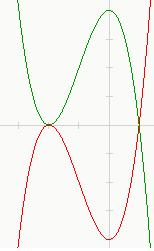
\includegraphics[scale=1]{img/Ungleichungen_Aufg4} 
Mit Berechnung von f(0)=-4 bekommt man wieder den richtigen Graphen, und somit direkt die L�sungsmenge $L=\lbrace x\in\R\mid x>1\rbrace$.\newline
\newline
\textbf{Aufgabe 5:}
\begin{center}
	$x^3+3x^2+3x+1<0$
\end{center}

\noindent Selbes Vorgehen wie bei der letzten Aufgabe: Zun�chst Bestimmung der Nullstellen ($x_{1,2,3}=-1$). Daraus ergeben sich jetzt wieder 2 m�gliche Graphen:
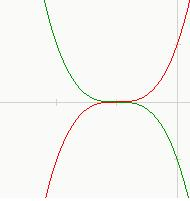
\includegraphics[scale=1]{img/Ungleichungen_Aufg5}
Mit f(0)=1 ergibt sich damit als L�sungsmenge $L=\lbrace x\in\R\mid x<-1\rbrace$.
